Das Programm ist in 3 wesentliche Schritte eingeteilt:

\begin{enumerate}
	\item Einlesen / Verteilen der Matrix
	\item Ermitteln der maximalen zusammenhängenden Komponenten im lokalen Bereich der Matrix
	\item Übermitteln der Ergebnisse an einen Nachbarn
\end{enumerate}

\subsection{Einlesen, Verteilen}

Nach dem Programmstart wird die Matrix vom Dateisystem des Root-Prozesses eingelesen. Dafür wird die Datei als Parameter beim Programmaufruf angegeben. Anschließend teilt der Root-Prozess die Matrix in möglichst gleich große Teile und verschickt diese an die anderen Prozesse im Cluster. In der aktuellen Programmversion teilt der Root-Prozess die Matrix immer in Streifen. Falls dabei die Anzahl der Matrix-Spalten nicht durch die Anzahl der Prozessoren teilbar ist, wird der Rest dem letzten Prozess zugeteilt (siehe Abb. \ref{fig:matrix_zerteilung} auf Seite \pageref{fig:matrix_zerteilung}).

\begin{figure}[tbhp]
	\centering
	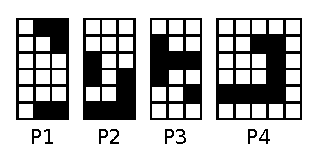
\includegraphics[width=0.7\textwidth]{images/matrix_split.eps}
	\caption{Beispiel für die Zerlegung einer Matrix zur Laufzeit}
	\label{fig:matrix_zerteilung}
\end{figure}

Durch diese Aufteilung kann ein Ungleichgewicht zwischen dem letzen und den restlichen Prozessen entstehen. Da der letzte Prozess aber auch derjenige ist, der am längsten auf seine Vorgänger warten muss, ensteht keine wesentliche Verzögerung im Programmablauf.

Eine zukünftige Version sollte außerdem auf die Eingabedimensionen der Matrix Rücksicht nehmen. Für den Fall, dass die Zeilenanzahl größer als die Spaltenanzahl ist ($m > n$), sollte das Programm die Matrix horizontal zerlegen, damit die Ränder möglichst klein bleiben.

\subsection{Ermitteln der lokalen Komponenten}

Im nächsten Schritt führt jeder Prozessor im Cluster den Kern-Algorithmus mit der empfangenen Matrix aus (siehe Abschnitt \ref{algorithm:find_components} auf Seite \pageref{algorithm:find_components}). Als Rückgabe erhält der Prozessor die Liste der gefunden Komponenten und die Ränder der Matrix. In den Rändern ist jeweils eine eindeutige Komponenten-Nummer gespeichert (siehe Abb. \ref{fig:find_result} auf Seite \pageref{fig:find_result}).

\begin{figure}[tbhp]
	\centering
	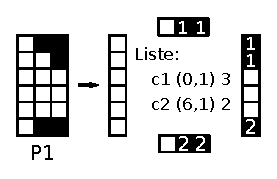
\includegraphics[width=0.6\textwidth]{images/find_result.eps}
	\caption{Beispiel für das (lokale) Ergebnis nach Ausführung der Komponenten-Ermittlung}
	\label{fig:find_result}
\end{figure}

\subsection{Übermittlung der Ergebnisse}

Im letzten Schritt müssen die Ergebnisse der lokalen Ermittlungen so zusammengefügt werden, dass die Komponenten, die durch die Zerteilung aufgeteilt wurden, wieder zusammengefügt werden.

Hierzu überträgt jeder Prozessor sein Ergebnis aus Schritt 2 an seinen direkten Nachbarn (Komponenten-Liste und der angrenzender Rand). Der Nachbar muss dann überprüfen, ob auf den beiden aneinanderliegenden Rändern Komponenten in direkter Nachbarschaft liegen. Falls das der Fall ist, muss eine der beiden Komponenten zur anderen hinzugefügt werden - hier ist nur die Größe relevant - und anschließend muss sie aus der Liste entfernt werden, um nicht doppelt zu erscheinen. Alle Komponenten aus der empfangenen Liste, die nicht mit eigenen Komponenten zusammenhängen werden in die eigene Liste übernommen.

In unserem Beispiel würde Prozessor 2 Komponente 1 und Komponente 2 von Prozessor 1 jeweils zu einer eigenen Komponente hinzufügen. Beide Komponenten würde anschließend gelöscht und nicht weiter zum nächsten Prozessor übertragen. Die eigenen Komponenten von Prozessor 2 wären dann 5 und 7 Pixel groß.

Nachdem die Ergebnisse schließlich beim letzten Prozessor angekommen sind und ausgewertet wurden, steht das Gesamtergebnis fest und wird ausgegeben.